\documentclass[journal,trans]{IEEEtran}
\usepackage[utf8]{inputenc}
\usepackage[spanish,es-tabla]{babel}
\usepackage[bottom]{footmisc}
\usepackage[hidelinks]{hyperref}
\usepackage[parfill]{parskip}
\usepackage[]{graphicx}
\usepackage[]{float}
\usepackage[]{caption}
\usepackage[]{multirow}
\usepackage[]{multicol}
\usepackage[]{siunitx}
\usepackage[]{tabularx}
\usepackage[]{amsmath}
\usepackage[]{textcomp, gensymb}
\usepackage[]{array}
\spanishdecimal{.}
\graphicspath{{Figures/}}
\hyphenation{op-tical net-works semi-conduc-tor}
\raggedbottom

\begin{document}

%\\\\\\\\\\\\\\\\\\\\\\\\\\\\\\\\\\\\\\\\\\\\\\
%Título
%\\\\\\\\\\\\\\\\\\\\\\\\\\\\\\\\\\\\\\\\\\\\\\

\title{Diseño, implementación y validación de una tarjeta de pruebas para el microcontrolador Siwa}

\renewcommand\IEEEkeywordsname{Palabras clave}

\author{ \rule{\linewidth}{0.5pt}\vspace{10pt}
\IEEEauthorblockN{Instituto Tecnológico de Costa Rica \\Escuela de Ingeniería Electrónica \\EL5610 Taller Integrador \\Prof. Luis Carlos Rosales Alpízar\\Brayan Barquero Madrigal$^{1}$, Yailyn Priscilla Campos Zamora$^{2}$, Fiorela Chavarria Castrillo$^{3}$, Jeffrey Salas Quiel$^{4}$\\brabarmad@estudiantec.cr$^{1}$, camposzamora@estudiantec.cr$^{2}$}, fchavarria@estudiantec.cr$^{3}$, jeffrey080203@estudiantec.cr$^{4}$}

\markboth{}%
{Shell \MakeLowercase{\textit{et al.}}: Bare Demo of IEEEtran.cls for Journals}

%\\\\\\\\\\\\\\\\\\\\\\\\\\\\\\\\\\\\\\\\\\\\\\
%Resumen y Palabras Clave
%\\\\\\\\\\\\\\\\\\\\\\\\\\\\\\\\\\\\\\\\\\\\\\

\IEEEtitleabstractindextext{%

\begin{abstract}
Resumen aquí...
\end{abstract}

\begin{IEEEkeywords}
Altium, PCB, Siwa.
\end{IEEEkeywords}}

\maketitle
\IEEEdisplaynontitleabstractindextext
\IEEEpeerreviewmaketitle

\setlength{\parindent}{1.27cm}
\setlength{\parskip}{0cm}


%\\\\\\\\\\\\\\\\\\\\\\\\\\\\\\\\\\\\\\\\\\\\\\
%Introducción
%\\\\\\\\\\\\\\\\\\\\\\\\\\\\\\\\\\\\\\\\\\\\\\

\section{Introducción}

%Explicar el contexto y los alcances del proyecto.

%\\\\\\\\\\\\\\\\\\\\\\\\\\\\\\\\\\\\\\\\\\\\\\
%Proceso de diseño
%\\\\\\\\\\\\\\\\\\\\\\\\\\\\\\\\\\\\\\\\\\\\\\

\section{Proceso de diseño}

%Explicar los pasos que se siguieron para diseñar la PCB.

%\\\\\\\\\\\\\\\\\\\\\\\\\\\\\\\\\\\\\\\\\\\\\\
%Proceso de fabricación
%\\\\\\\\\\\\\\\\\\\\\\\\\\\\\\\\\\\\\\\\\\\\\\

\section{Proceso de fabricación}

%Explicar los pasos de fabricación y los errores que se encontraron y las causas posibles.

\subsection{Perforado}
Una vez terminado el diseño en Altium, se exportan los archivos para la fabricación de la PCB. A partir de estos,
se realiza el perforado de la placa de cobre para obtener los orificios pasantes (\text{through-hole}) y las vías. En la figuras
 \ref{fig:drilling_1} y \ref{fig:drilling_2} se observan el plano de referencia para el perforado y la placa ya perforada, respectivamente. 

\begin{figure}[H]
    \centering
    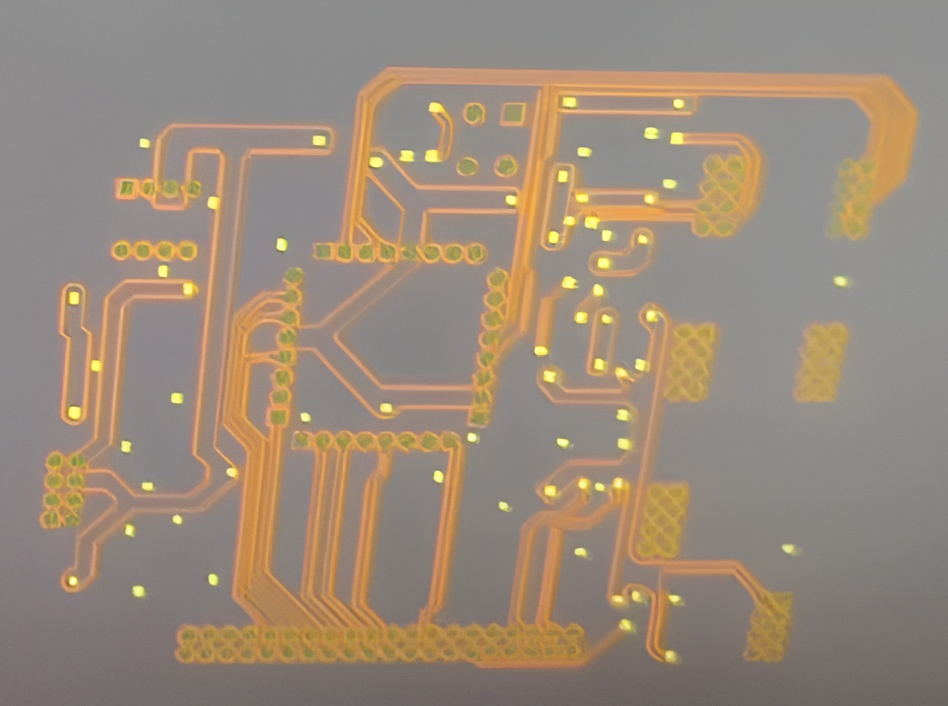
\includegraphics[width=0.4\textwidth]{Figures/making/1_fabricacion_drilling.png}
    \caption{Plano de referencia para el perforado.}
    \label{fig:drilling_1}
\end{figure}

\begin{figure}[H]
    \centering
    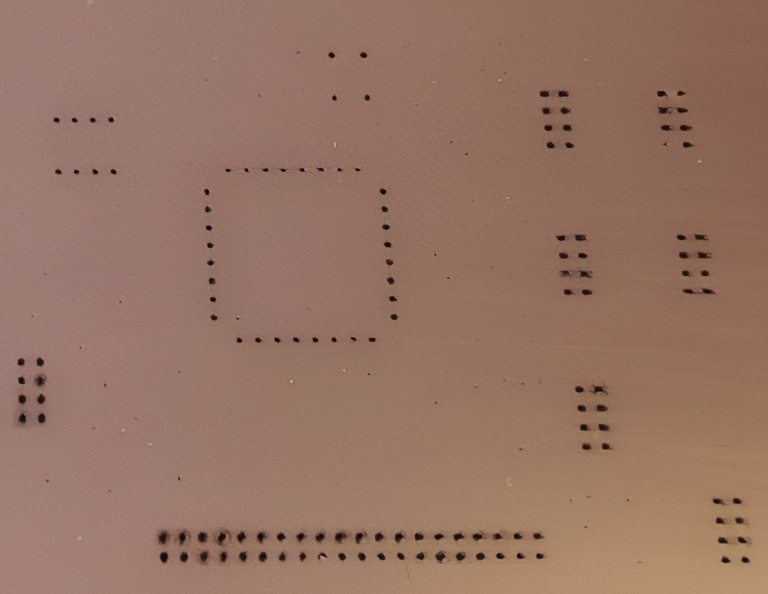
\includegraphics[width=0.4\textwidth]{Figures/making/3_fabricacion_drilling.png}
    \caption{Placa perforada.}
    \label{fig:drilling_2}
\end{figure}

\subsection{Metalización de orificios}

Después del perforado, se realiza la metalización de los orificios para permitir la conexión eléctrica entre las capas de la PCB. 
Primero, se lava la placa perforada utilizando agua tibia con el fin de remover cualquier residuo. Luego, se realiza un baño en 
carbón activado, para que las paredes de los orificios queden eléctricamente conductoras, ya que despues del perforado, estas son
de material dieléctrico (figura \ref{fig:carbon_bath}). 

\begin{figure}[H]
    \centering
    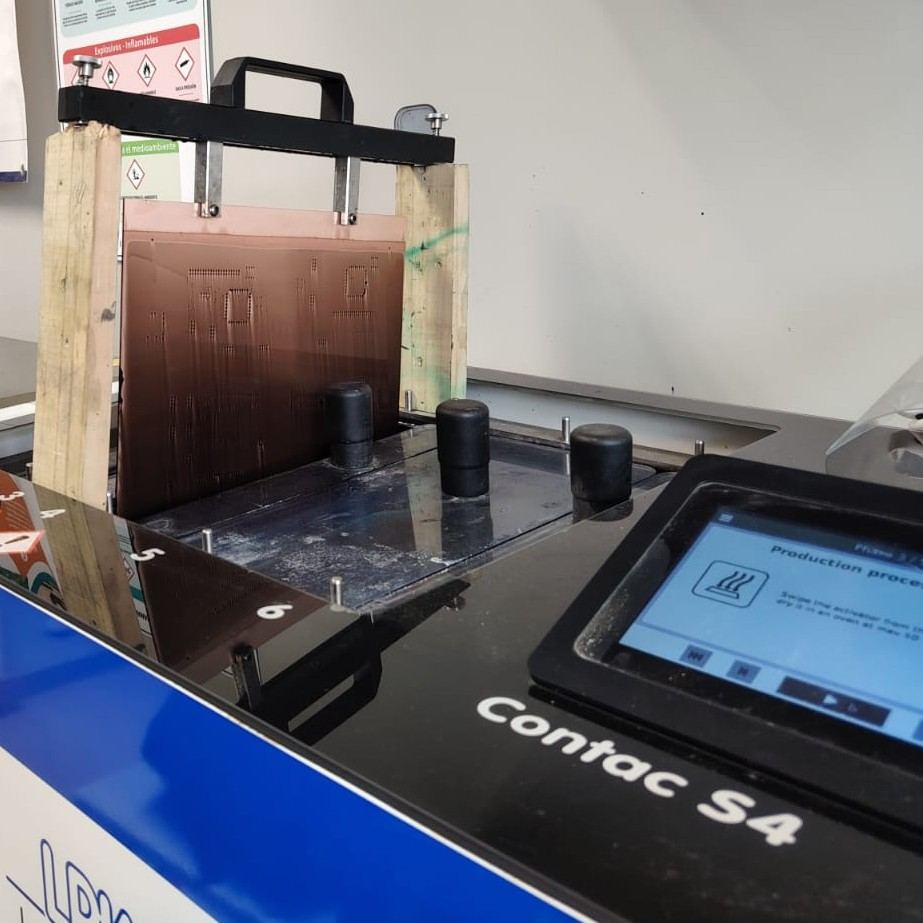
\includegraphics[width=0.4\textwidth]{Figures/making/6_fabricacion_baño_carbon.jpeg}
    \caption{Baño en carbón activado para metalizar los orificios.}
    \label{fig:carbon_bath}
\end{figure}

Después de este proceso, se utiliza un horno para secar la placar y fijar
el carbón activado obteniendo el resultado mostrado en la figura \ref{fig:carbon_bath_result}.

\begin{figure}[H]
    \centering
    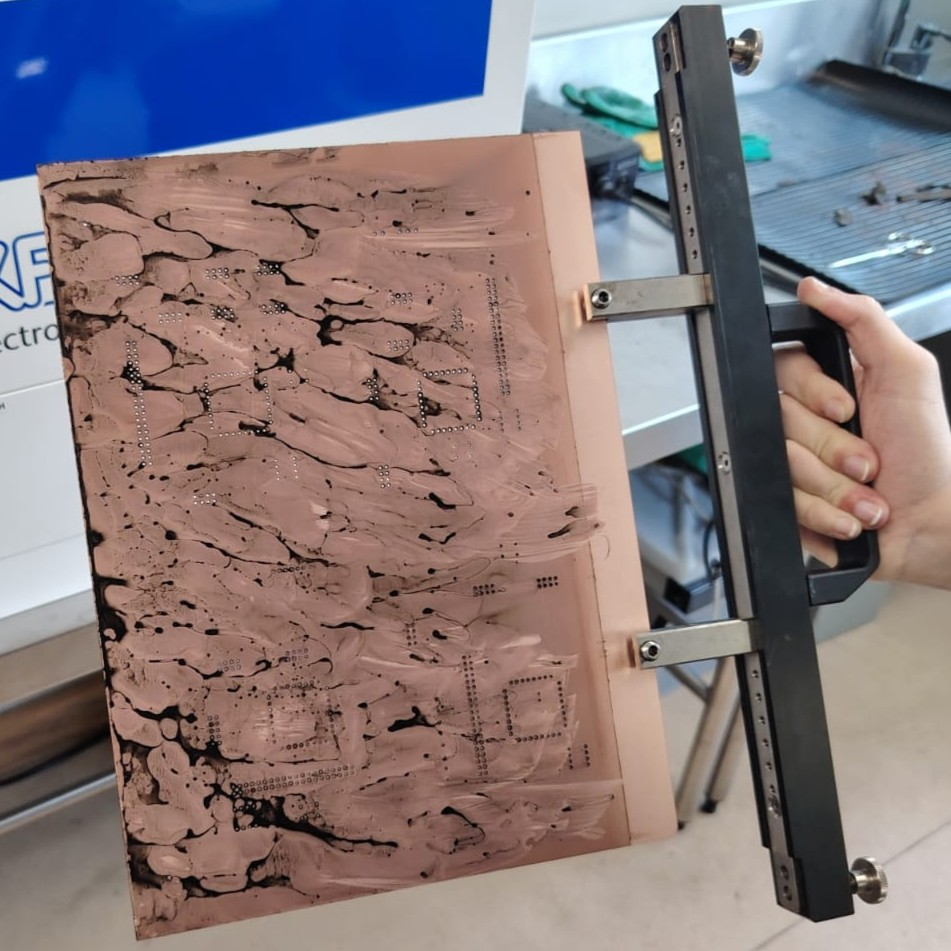
\includegraphics[width=0.4\textwidth]{Figures/making/8_fabricacion_placa_seca_carbon.jpeg}
    \caption{Resultado después de secar la placa y fijar el carbón activado.}
    \label{fig:carbon_bath_result}
\end{figure}

A continuación, se realiza un baño en ácido sulfúrico para galvanizar los orificios, es decir, 
cubrirlos con una capa de metal (figura \ref{fig:acid_bath}).

\begin{figure}[H]
    \centering
    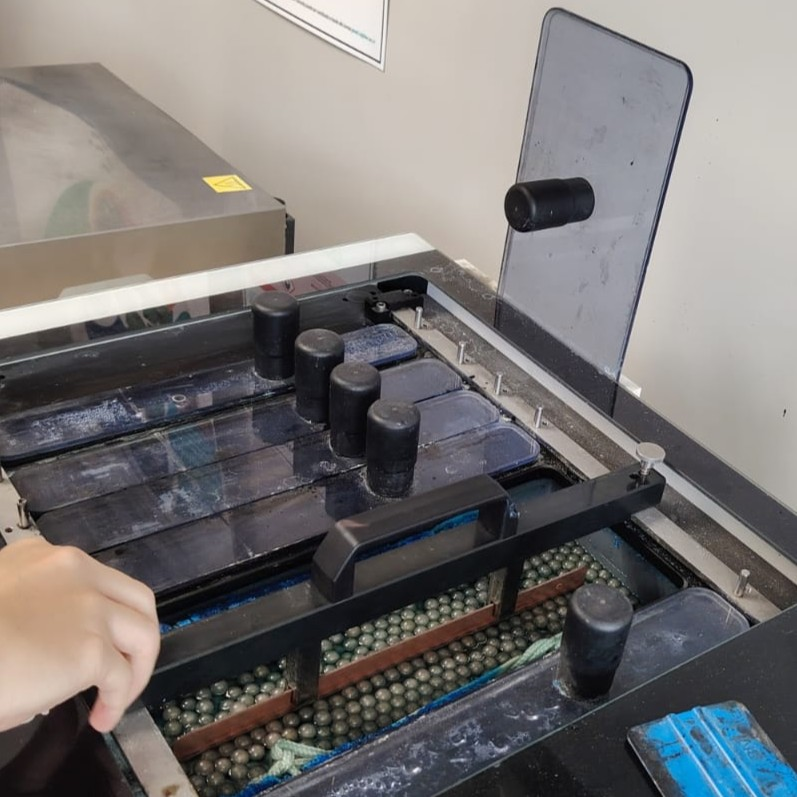
\includegraphics[width=0.4\textwidth]{Figures/making/9_fabricacion_baño_acido.jpeg}
    \caption{Baño en ácido sulfúrico para galvanizar los orificios.}
    \label{fig:acid_bath}
\end{figure}

Después se limpia la placa con agua para obtener el resultado mostrado en la figura \ref{fig:acid_bath_result}.

\begin{figure}[H]
    \centering
    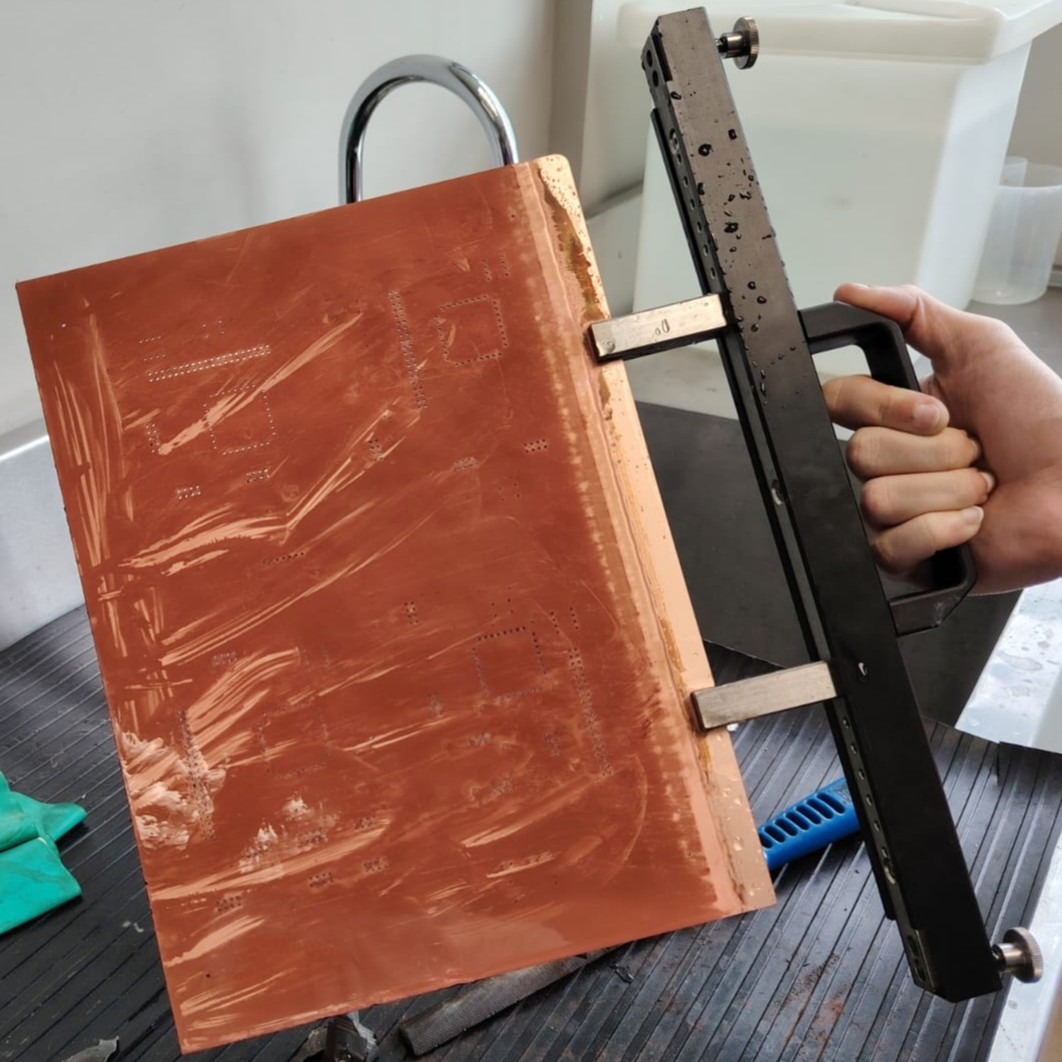
\includegraphics[width=0.4\textwidth]{Figures/making/11_fabricacion_lavado_final.jpeg}
    \caption{Resultado después de del baño en ácido sulfúrico y de limpiar la placa con agua.}
    \label{fig:acid_bath_result}
\end{figure}

\subsection{Recubrimiento y curado}

Se parte de la placa perforada, sobre la que se aplica una fotorresina 
que se expone a luz UV a través del diseño del circuito. Las zonas no endurecidas se disuelven y 
el cobre expuesto se elimina químicamente, dejando solo las pistas. Luego se perforan los orificios,
se aplica la máscara de soldadura verde que protege el cobre y deja al descubierto solo los pads,
y finalmente se imprime la serigrafía blanca con las referencias de los componentes. El resultado es el
que se muestra en la figura \ref{fig:coating}.

\begin{figure}[H]
    \centering
    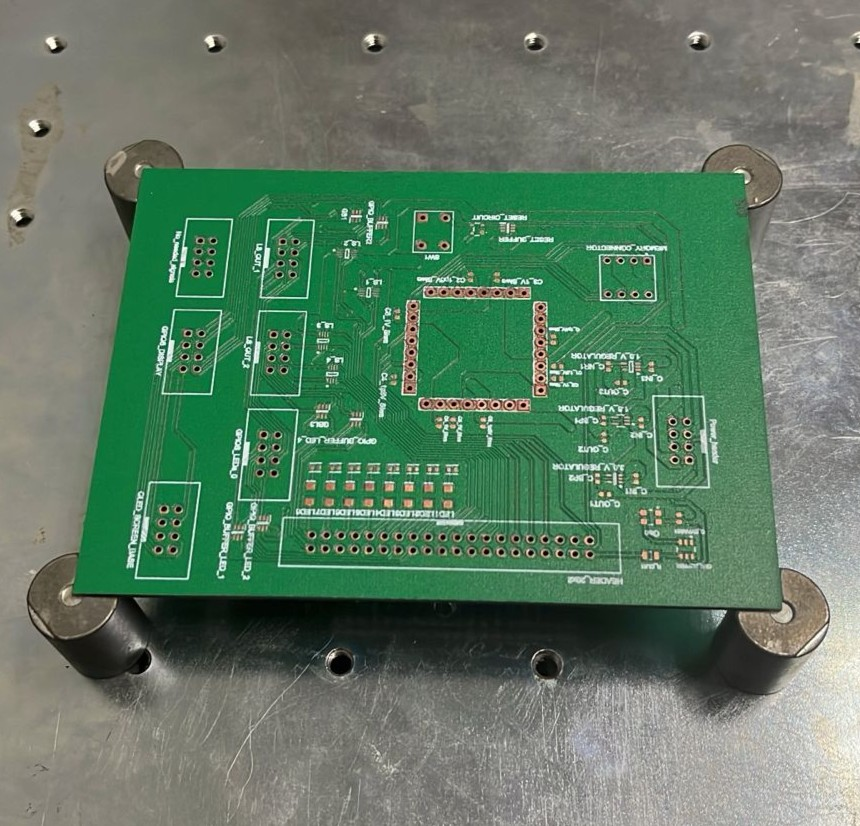
\includegraphics[width=0.4\textwidth]{Figures/making/12_fabricacion_resultado_impresion.jpeg}
    \caption{Resultado después de aplicar la máscara de soldadura y la serigrafía.}
    \label{fig:coating}
\end{figure}

\subsection{Soldadura de montaje superficial}

Con ayuda de un \textit{stencil} se aplica manualmente la pasta de soldadura sobre los pads de la placa (ver figura \ref{fig:stencil}), 
luego se retira el \textit{stencil} (ver figuras \ref{fig:stencil_removed} y \ref{fig:stencil_removed2}).

\begin{figure}[H]
    \centering
    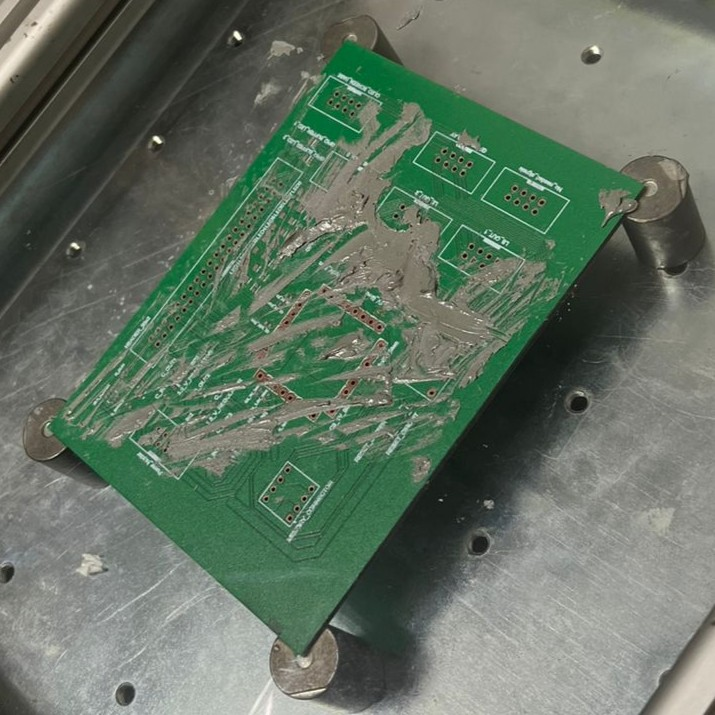
\includegraphics[width=0.4\textwidth]{Figures/making/13_pasta_soldadura.jpeg}
    \caption{Aplicación de la pasta de soldadura usando un \textit{stencil}.}
    \label{fig:stencil}
\end{figure}

\begin{figure}[H]
    \centering
    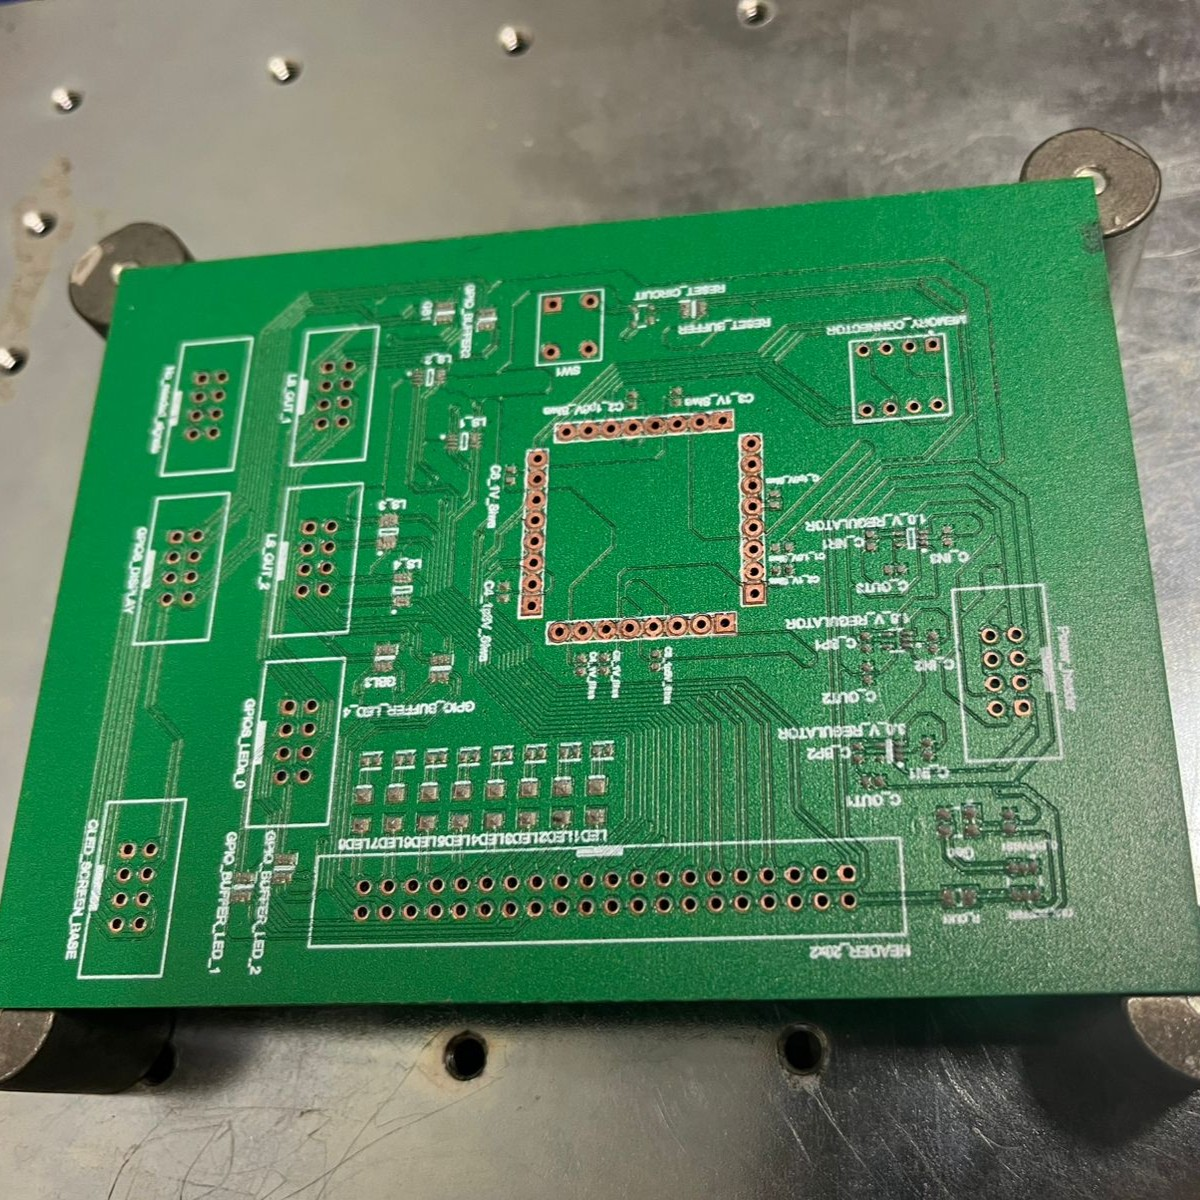
\includegraphics[width=0.4\textwidth]{Figures/making/14_pasta_soldadura_aplicada.jpeg}
    \caption{Resultado después de retirar el \textit{stencil}.}
    \label{fig:stencil_removed}
\end{figure}

\begin{figure}[H]
    \centering
    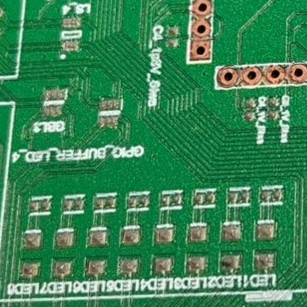
\includegraphics[width=0.4\textwidth]{Figures/making/14_pasta_soldadura_aplicada_close_up.jpeg}
    \caption{Detalle del resultado después de retirar el \textit{stencil}.}
    \label{fig:stencil_removed2}
\end{figure}

Una vez que los pads están cubiertos con la pasta de soldadura, se colocan los componentes de montaje superficial
manualmente con ayuda de una máquina \textit{pick and place} (ver figuras \ref{fig:pick_and_place} y \ref{fig:pick_and_place_close_up}).

\begin{figure}[H]
    \centering
    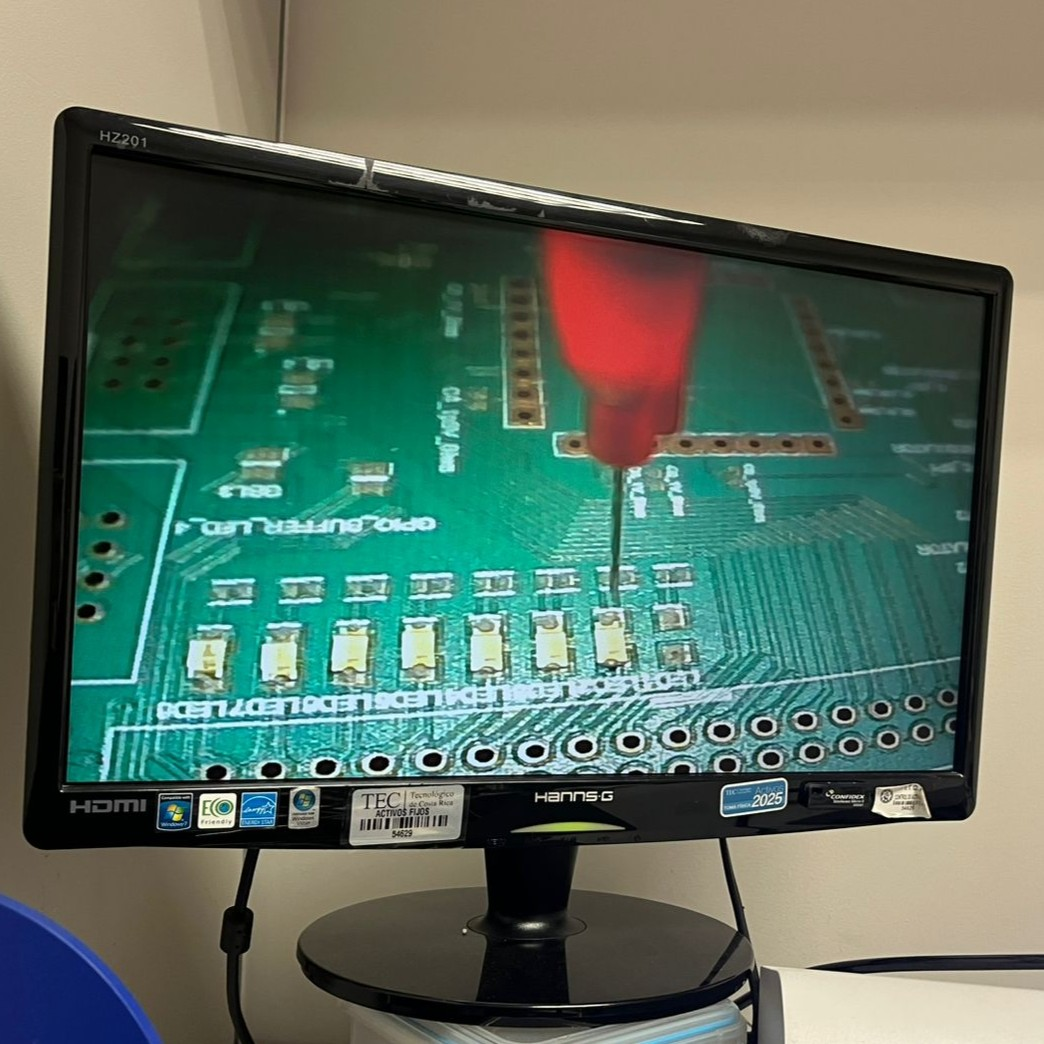
\includegraphics[width=0.4\textwidth]{Figures/making/15_aplicacion_pick_place.jpeg}
    \caption{Colocación de los componentes de montaje superficial usando la máquina \textit{pick and place}.}
    \label{fig:pick_and_place}
\end{figure}

\begin{figure}[H]
    \centering
    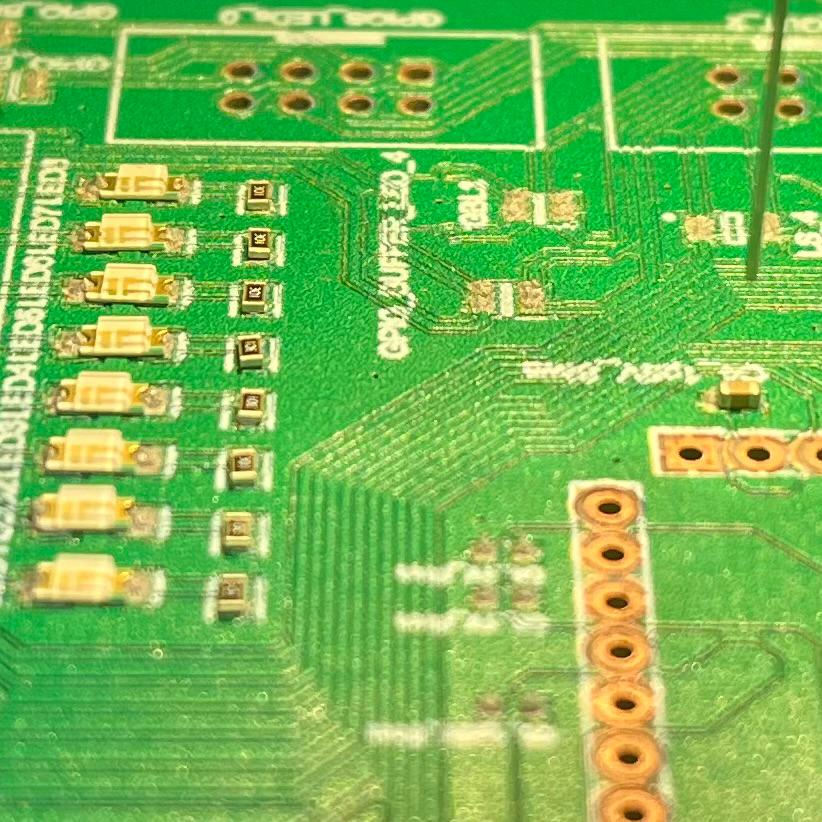
\includegraphics[width=0.4\textwidth]{Figures/making/15_aplicacion_pick_place_close_up.jpeg}
    \caption{Detalle de la colocación de los componentes de montaje superficial usando la máquina \textit{pick and place}.}
    \label{fig:pick_and_place_close_up}
\end{figure}

Una vez que se han colocado todos los componentes de montaje superficial, se introduce la placa en un horno para fijar la soldadura (figura \ref{fig:horneado}). 

\begin{figure}[H]
    \centering
    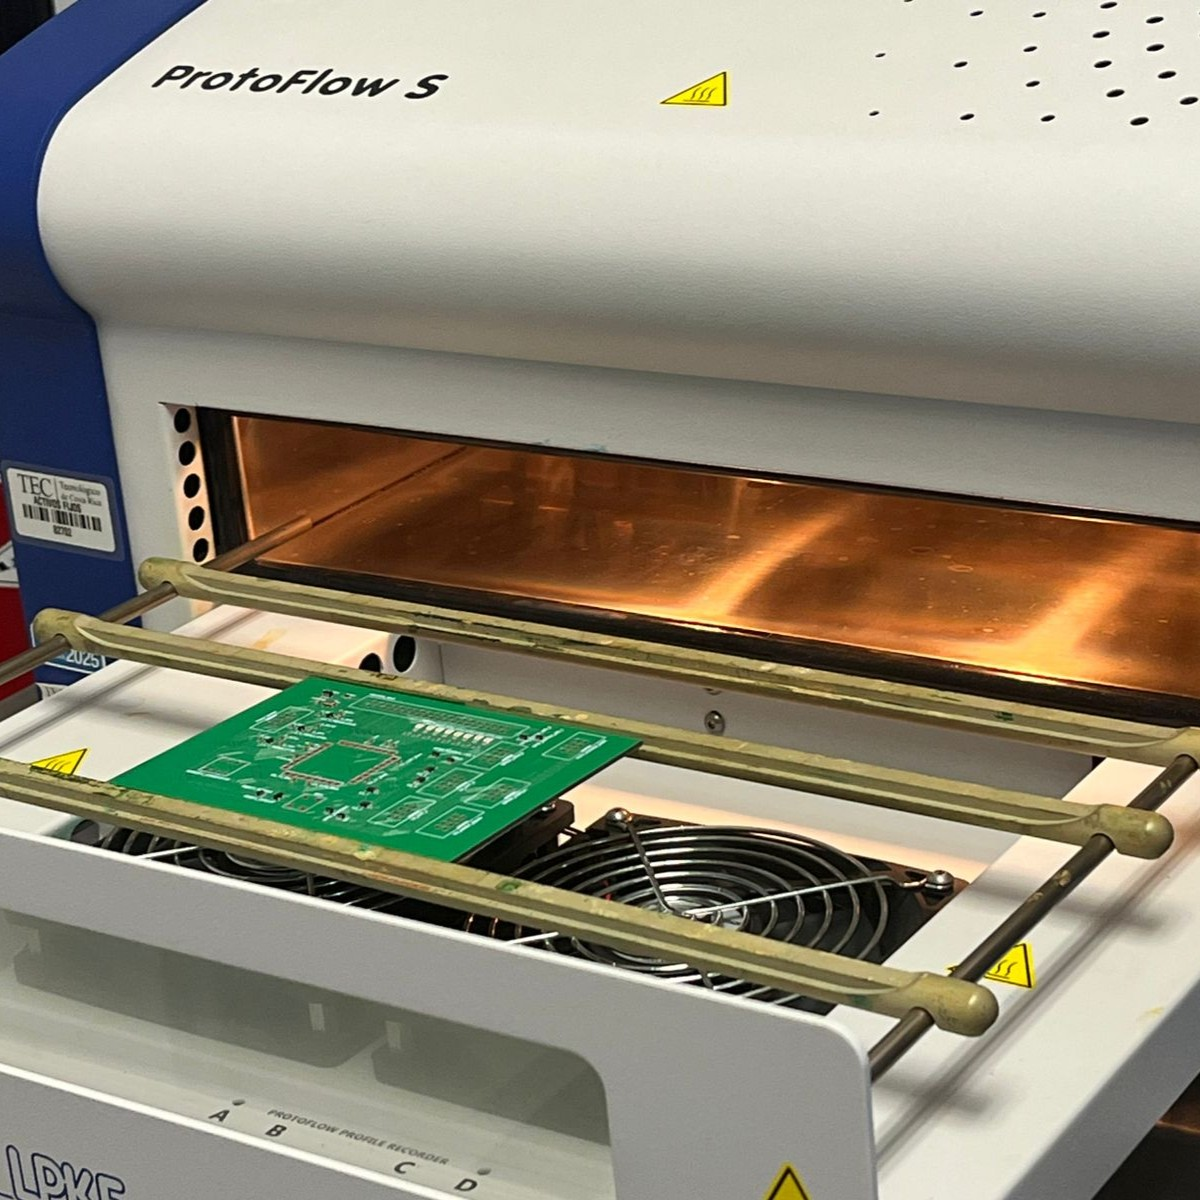
\includegraphics[width=0.4\textwidth]{Figures/making/16_horneado.jpeg}
    \caption{Horneado de la placa para fijar la soldadura de los componentes de montaje superficial.}
    \label{fig:horneado}
\end{figure}

\subsection{Soldadura de componentes pasantes}

Después de fijar los componentes de montaje superficial, se procede a soldar los componentes pasantes manualmente 
con una estación de soldadura (figura \ref{fig:fabricacion_soldadura}), obteniendo el resultado mostrado en la figura \ref{fig:fabricacion_soldadura_resultado}.

\begin{figure}[H]
    \centering
    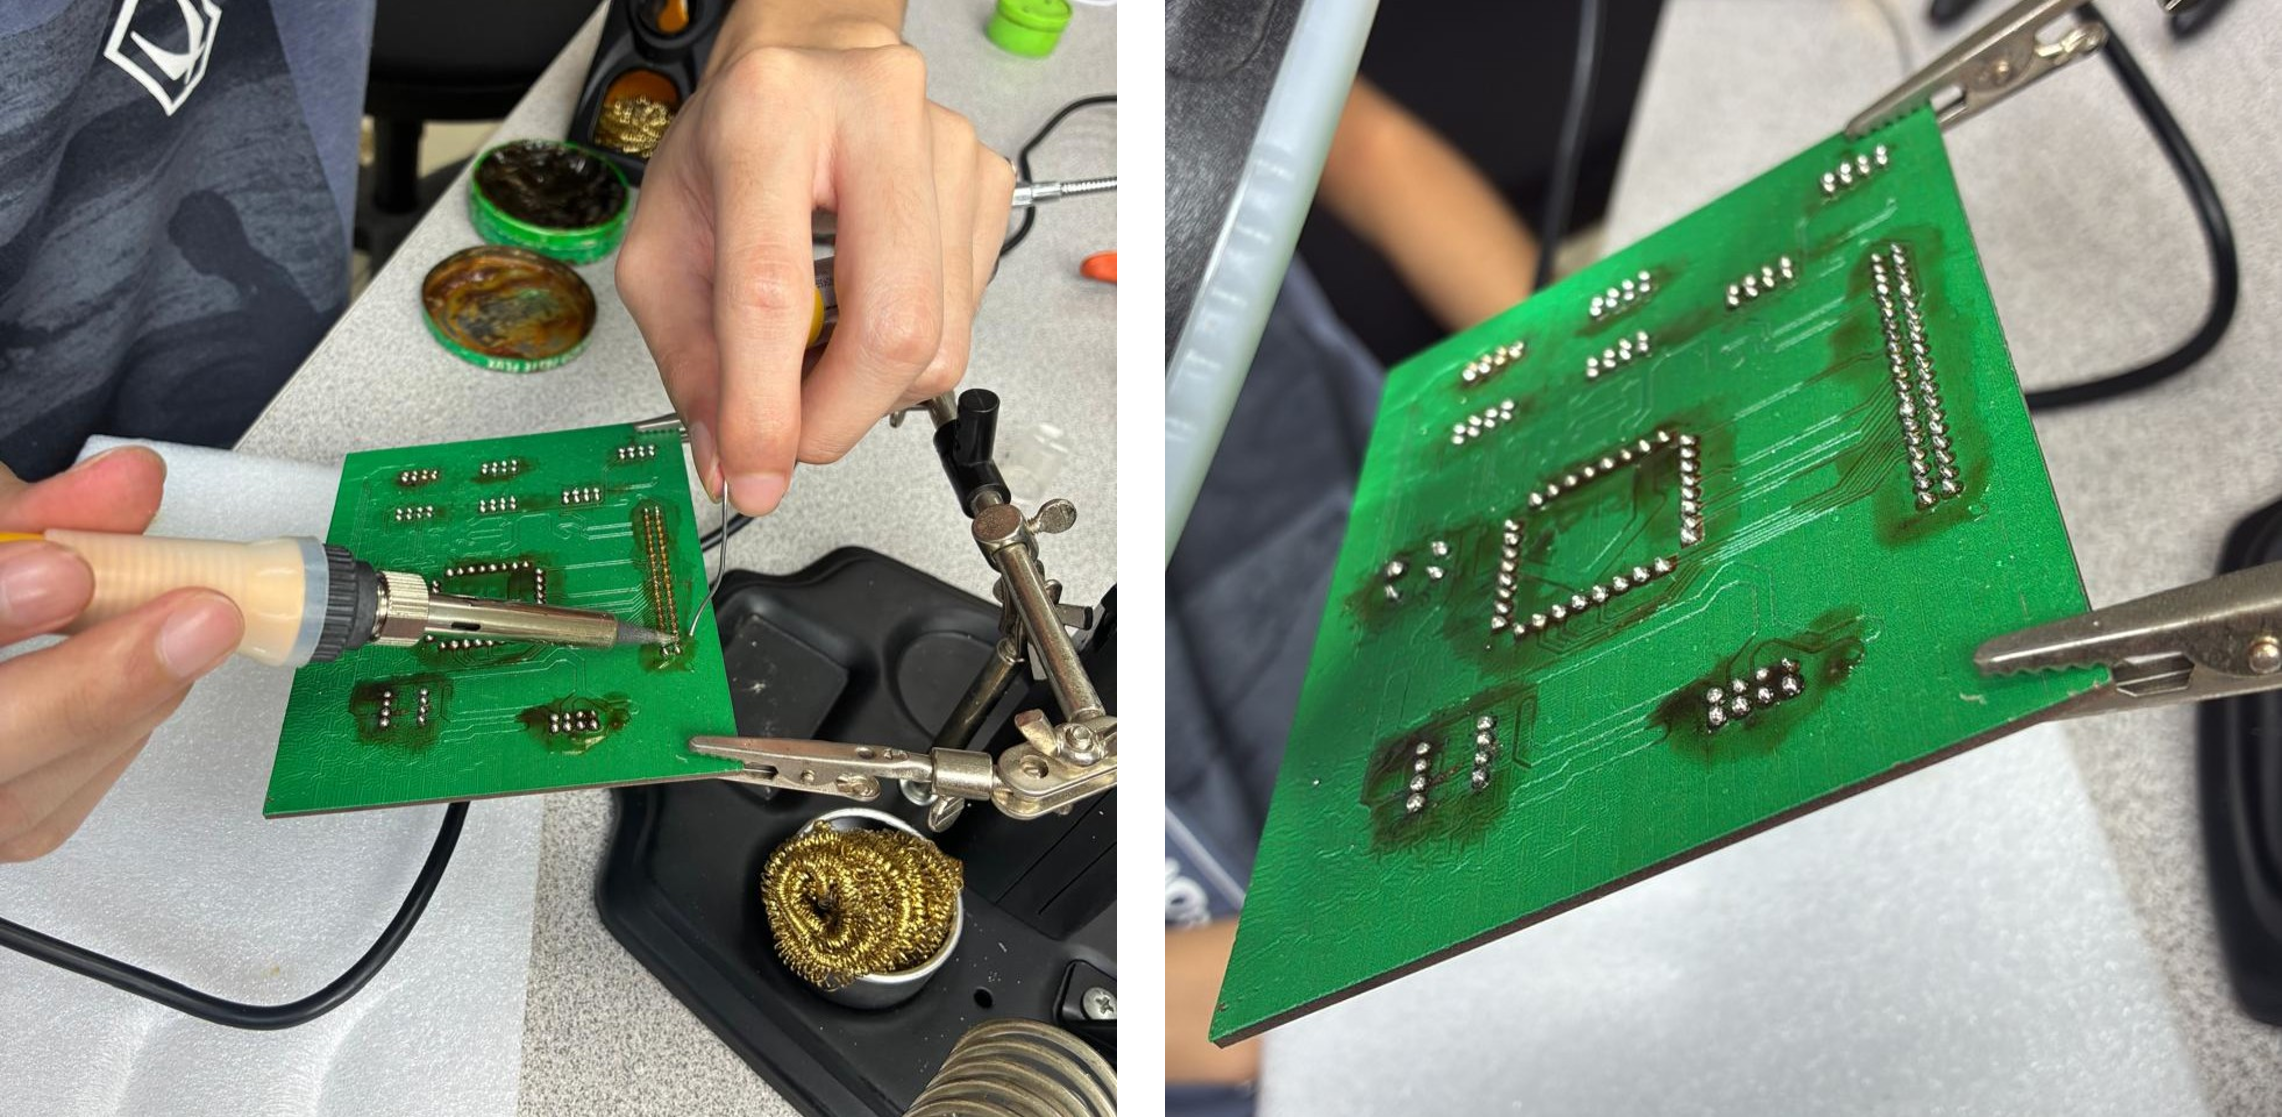
\includegraphics[width=0.4\textwidth]{Figures/making/fabricacion_soldadura.png}
    \caption{Proceso de soldadura de los componentes pasantes.}
    \label{fig:fabricacion_soldadura}
\end{figure}

\begin{figure}[H]
    \centering
    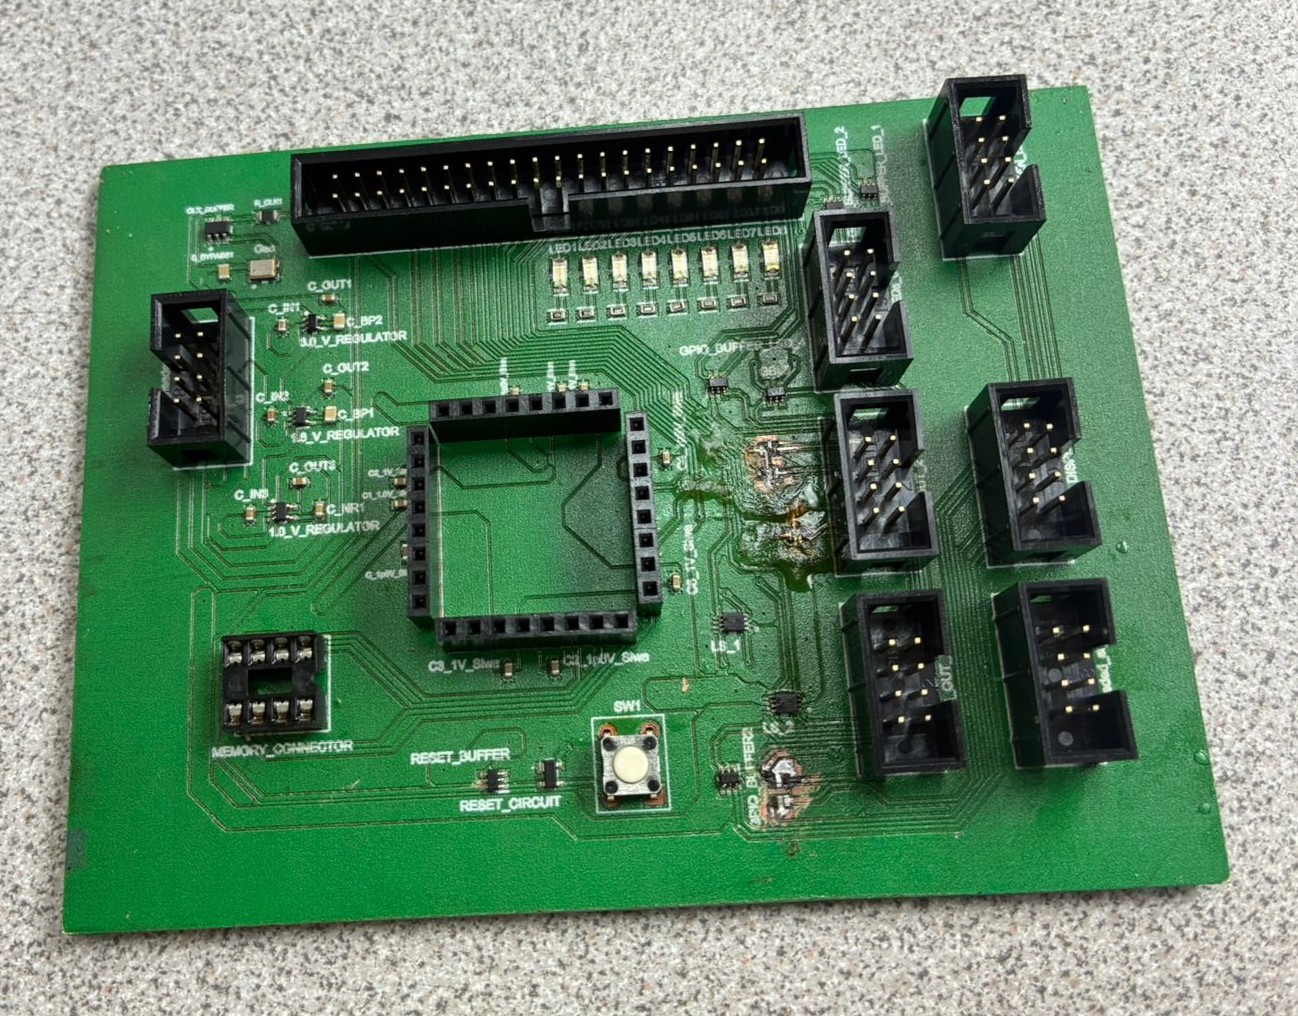
\includegraphics[width=0.4\textwidth]{Figures/making/19_soldadura_componentes.jpeg}
    \caption{Resultado de la placa con los componentes pasantes soldados.}
    \label{fig:fabricacion_soldadura_resultado}
\end{figure}

%\\\\\\\\\\\\\\\\\\\\\\\\\\\\\\\\\\\\\\\\\\\\\\
%Proceso de validación
%\\\\\\\\\\\\\\\\\\\\\\\\\\\\\\\\\\\\\\\\\\\\\\

\section{Proceso de validación}

%¿Cómo se prueba la integridad de la tarjeta? Explicar el procedimiento seguido.

%\\\\\\\\\\\\\\\\\\\\\\\\\\\\\\\\\\\\\\\\\\\\\\
%Proceso operativo
%\\\\\\\\\\\\\\\\\\\\\\\\\\\\\\\\\\\\\\\\\\\\\\

\section{Proceso operativo}

%¿Cómo fue organizado el trabajo y la asignación de tareas y responsabilidades entre los miembros del grupo?

%\\\\\\\\\\\\\\\\\\\\\\\\\\\\\\\\\\\\\\\\\\\\\\
%Conclusiones
%\\\\\\\\\\\\\\\\\\\\\\\\\\\\\\\\\\\\\\\\\\\\\\

\section{Conclusiones}

%Al menos 1 por miembro del equipo.

El proceso de fabricación de la PCB es propenso a errores debido a la manualidad de los pasos involucrados,
desde la aplicación de la pasta de soldadura con el \textit{stencil} hasta la colocación de los componentes de montaje superficial
con ayuda de la máquina de \textit{pick and place}, donde se debe estimar la posición y orientación de cada componente con precisión.

%\\\\\\\\\\\\\\\\\\\\\\\\\\\\\\\\\\\\\\\\\\\\\\
%Referencias
%\\\\\\\\\\\\\\\\\\\\\\\\\\\\\\\\\\\\\\\\\\\\\\

\begin{thebibliography}{1} 
    \bibitem{Clive} C. Maxfield, The design warrior's guide to FPGAs, 1st ed. Amsterdam: Newnes/Elsevier, 2004.
\end{thebibliography}

\end{document}